\subsection{Pipeline View}
\label{sec:pipeline}
Pipeline view provides a direct visual representation of the three stages (encoder, attention, classifier) of the model. In the proposed tool, we allow the model parameter to be updated (via an optimization) to correct a prediction error (\textbf{T3}). The pipeline view, by visualizing the aggregated gradient distribution, informs the user on the how each stage of the model responses to the optimization.

There are many ways to update the model to correct a prediction. A simple way to achieve it is applying standard backpropagation that overfits to the example. However, without any constraint, the update step may alter the model in unexpected ways.
% \shusen{what is the benefit of using mira?}
Instead, we adopt the same idea in \emph{Margin-infused relaxed algorithm (MIRA)}~\cite{CrammerSinger2003}, where we regulate the optimization with the L2-norm of the parameter change. Therefore, in the proposed tool, we obtain the target parameters by the following:
\begin{equation}
\underset{w'}{\mathrm{argmin}}( C \mathbb{J}(\mathbf{W}') + ||\mathbf{W}' - \mathbf{W}||^2)
\end{equation}
where $\mathbb{J}(\mathbf{W})$ is the loss function of the neural model, $\mathbf{W}$ is the original model's parameters taken as constant, $\mathbf{W}'$ is the parameters to update, and $C$ is the weighting term, which determines whether we intended to emphasis more on obtaining better fitting or deviating less from the original model. Due to the nonconvex nature of the neural networks, we use SGD to optimize the above combined loss function.
%
Under this formation, we try to find a good approximation to the newly assigned label, while still maintaining relatively small change with respect to the original model.

As illustrated in Fig.~\ref{fig:pipelineView},
the optimization hyperparameters are shown in Fig.~\ref{fig:pipelineView}(a). Each of the stages is illustrated by a glyph (Fig.~\ref{fig:pipelineView}(b)), in which the user can enable or disable its parameter update by click on the parameter bar (the legend about its state is shown in Fig.~\ref{fig:pipelineView}(d) ). In Fig.~\ref{fig:pipelineView}(c), we select whether if we want to use current update setting as displayed or try all the configuration combination (i.e., each stage can either be enabled or disabled for the three stage, therefore, there are $8$ combinations in total, $7$ if discard the case where all stages are not updated).

\begin{figure}[htbp]
\centering
\vspace{-2mm}
 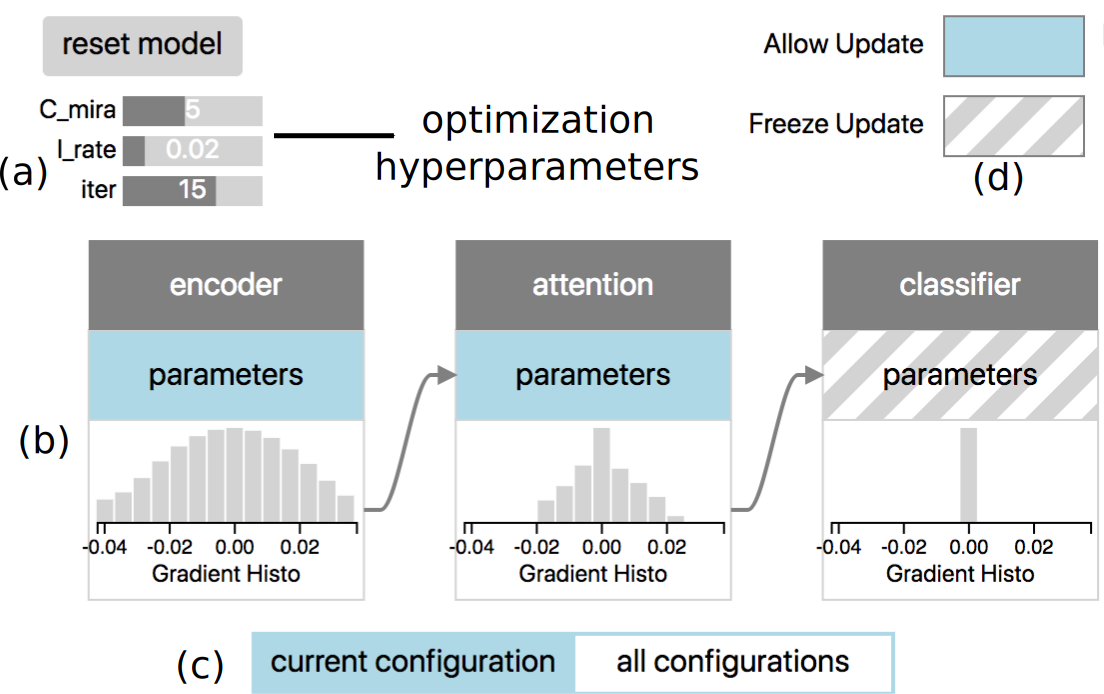
\includegraphics[width=1.0\linewidth]{pipelineView}
 \caption{
 The pipeline view provides the visual representation of three stages (encoder, attention, classifier) model. In the proposed tool, we allow the model parameter to be updated to correct a prediction error. The pipeline view, by showing the aggregated gradient distribution, informs the user about the how different part of the model response to the optimization.
 %
 The optimization hyperparameters are shown in (a), each of the stages is illustrated in (b), where the user can click on the parameter bar to enable or disable its update (the legend about its state is shown in (d) ). In (c), we select whether if we want to use current update setting as displayed or try all the possible configuration combination (i.e., each stage's parameter update can be enabled or disabled).
 }
\label{fig:pipelineView}
\end{figure}

% \textbf{Margin-Infused Relaxed Algorithm (MIRA)}
